\documentclass[11pt]{article}
\usepackage{geometry}                % See geometry.pdf to learn the layout options. There are lots.
\geometry{letterpaper}                   % ... or a4paper or a5paper or ... 
%\geometry{landscape}                % Activate for for rotated page geometry
%\usepackage[parfill]{parskip}    % Activate to begin paragraphs with an empty line rather than an indent
\usepackage{graphicx}
\usepackage{amssymb}
\usepackage{epstopdf}
\DeclareGraphicsRule{.tif}{png}{.png}{`convert #1 `dirname #1`/`basename #1 .tif`.png}


%%
%% TIKZ for drawing DAGs (not sure how much of the below is necessary)
%%

\usepackage{tikz}
\usepackage{tkz-graph}
\usetikzlibrary{shapes,arrows}

\newcommand{\entrynode}[1]{
  \SetVertexNormal[Shape      = circle,
                   FillColor  = black,
                   LineWidth  = 0pt,
                   MinSize    = 0pt]
  \Vertex[L={\tiny\,}]{#1}
  \SetVertexNormal[Shape      = circle,
                   FillColor  = white,
                   LineWidth  = 2pt]
}

\SetUpEdge[lw         = 1.5pt,
           color      = black,
           labelcolor = white,
           labeltext  = red,
           labelstyle = {sloped,draw,text=blue}]

\tikzset{node distance = 2cm}




\title{Anonymity in XIA: Developer Tools and User Control}
\author{Nicolas Feltman and David Naylor}
\date{}                                           


\begin{document}
\maketitle


DAG Example:\\
\begin{center}
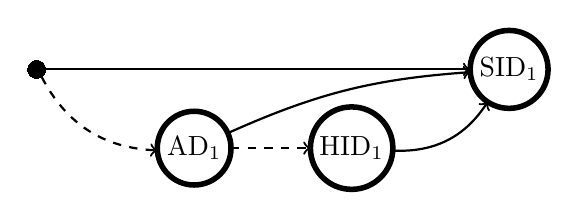
\begin{tikzpicture}
  \entrynode{A}
  \Vertex[x=6,y=0,L=SID$_1$]{B}
  \Vertex[x=2,y=-1,L=AD$_1$]{C}
  \Vertex[x=4,y=-1,L=HID$_1$]{D}
  \tikzstyle{EdgeStyle}=[->]
  \Edge(A)(B)
  \tikzstyle{EdgeStyle}=[dashed, bend right, ->]
  \Edge(A)(C)
  \tikzstyle{EdgeStyle}=[bend left=10, ->]
  \Edge(C)(B)
  \tikzstyle{EdgeStyle}=[dashed, ->]
  \Edge(C)(D)
  \tikzstyle{EdgeStyle}=[bend right, ->]
  \Edge(D)(B)
\end{tikzpicture}
\end{center}


\section{Introduction}
\subsection{Anonymity}
\subsection{XIA}


\section{Levels of Anonymity}


\section{Approach: Proxies}


\section{Approach: Temporary Service IDs}


\section{An API for Developers}
As we have discussed above, XIA allows for simple, if not elegant, ways to employ techniques for anonymization. For instance, we explored how an application can achieve fine-grain control over the use of a proxy service through DAG manipulation. We also proposed the use of temporary SIDs as pseudonyms.

Both of these strategies incorporate anonymity by leveraging core features of XIA. Thus, it is both possible and useful to a standard set of tools implementing these techniques to application developers --- it would be silly for each developer to implement his/her own functions for adding a proxy service to all outgoing DAGs, for example.

We have implemented these tools in the form of the XAnonSocket API, an extension to the XSocket API. (The XSocket API, as the name suggests, allows developers to communicate with sockets over XIA, much like network applications today use TCP or UDP sockets.) The XAnonSocket API allows developers to specify how they want to achieve anonymity (i.e., by routing traffic through a proxy of their choice) just once, after which they can send packets using the specified service with no extra effort. In \S~\ref{sec:api-interface} we present the interface of the XAnonSocket API.

\subsection{API Interface}
\label{sec:api-interface}

\begin{center}
	\begin{tabular}{l p{7cm}}
	\textbf{Function} 	&	\textbf{Description}\\
	\hline
	\texttt{XAnonSocket()} & Creates an anonymous XIA socket\\
	\texttt{XAnonRegisterAnonymizer(sock, dag)} & Specifies the DAG of an anonymization (e.g., proxy) service all packets sent through \texttt{sock} should be routed through\\
	\texttt{XAnonUseTempSID(sock, duration)} & Future packets should be sent from a temporary SID with HID elided. A new SID is generated after \texttt{duration} seconds\\
	\texttt{XAnonConnect(sock, dag)} & Connect to \texttt{ddag} with current anonymization settings\\
	\texttt{XAnonSend(sock, payload)} & Sends a packet with current anonymization settings\\
	\texttt{XAnonGetStatus(sock)} & Retrieves the current anonymization settings for \texttt{sock}\\
	\hline
	\end{tabular}
\end{center}


\section{Example Application: Web Browser}

\end{document}  